% ============================================================
% Chapter 6: Markov Chain Monte Carlo Methods
% Lectures on Monte Carlo Theory — Leskelä & Vihola
% ============================================================
\documentclass[aspectratio=169,10pt]{beamer}
\usetheme{Madrid}
\usecolortheme{seahorse}

\usepackage{amsmath,amssymb,amsthm}
\usepackage{mathtools}
\usepackage{bm}
\usepackage{xcolor}
\usepackage{booktabs}
\usepackage{graphicx}
\usepackage{listings}
\usepackage{tikz}
\usetikzlibrary{arrows.meta,positioning,shapes}

\graphicspath{{figures/}}

\lstdefinestyle{python}{
  language=Python,
  basicstyle=\ttfamily\scriptsize,
  numbers=left,
  numberstyle=\tiny\color{gray},
  frame=single,
  backgroundcolor=\color{gray!7},
  keywordstyle=\color{blue!70!black}\bfseries,
  commentstyle=\color{green!50!black}\itshape,
  stringstyle=\color{red!60!black},
  breaklines=true,
  showstringspaces=false,
  tabsize=4,
}

\setbeamertemplate{footline}[frame number]
\setbeamertemplate{navigation symbols}{}

\newcommand{\PP}{\mathbb{P}}
\newcommand{\EE}{\mathbb{E}}
\newcommand{\RR}{\mathbb{R}}
\newcommand{\ZZ}{\mathbb{Z}}
\newcommand{\dTV}{d_{\mathrm{TV}}}
\newcommand{\bfP}{\mathbf{P}}
\newcommand{\bfQ}{\mathbf{Q}}
\newcommand{\bfC}{\mathbf{C}}
\newcommand{\bfZ}{\mathbf{Z}}
\newcommand{\bff}{\mathbf{f}}
\newcommand{\bfpi}{\bm{\pi}}
\newcommand{\bfmu}{\bm{\mu}}

\title[Chapter 6: MCMC]{Chapter 6: Markov Chain Monte Carlo Methods}
\subtitle{Lectures on Monte Carlo Theory}
\author{Leskelä \& Vihola}
\date{}

% ============================================================
\begin{document}
% ============================================================

\begin{frame}
  \titlepage
\end{frame}

\begin{frame}{Chapter Overview}
  \tableofcontents
\end{frame}

% ============================================================
\section{6.1 Introduction}
% ============================================================

\begin{frame}{6.1 Introduction: Motivation}
  \textbf{Goal:} Estimate $I = \mathbb{E}f(Y)$ or $I = \mathbb{E}Y$ where $Y \sim \pi$.

  \medskip
  \textbf{Standard Monte Carlo:} Generate independent samples $Y_1,\ldots,Y_R \sim \pi$, use
  \[
    \hat{Y}_R = \frac{1}{R}\sum_{i=1}^R f(Y_i) \approx I.
  \]

  \begin{block}{The Problem}
    In many applications $\pi$ is \textbf{intractable}:
    \begin{itemize}
      \item The state space $\mathcal{S}$ is exponentially large (e.g.\ $|\mathcal{S}| = 2^d$).
      \item Direct sampling requires a normalizing constant $z_\lambda$ that is unknown.
      \item Example: $\pi_\sigma = \frac{1}{z_\lambda} e^{\lambda f(\sigma)}$ (Gibbs/Boltzmann distribution).
    \end{itemize}
  \end{block}

  \begin{block}{MCMC Solution}
    Construct a \textbf{Markov chain} $(X_n)$ whose stationary distribution \emph{is} $\pi$.
    Then
    \[
      \hat{Y}_R = \frac{1}{R}\sum_{j=1}^R f(X_j) \xrightarrow{R\to\infty} I \quad \text{(ergodic theorem)}.
    \]
  \end{block}
\end{frame}

\begin{frame}{6.1 Introduction: Running Example}
  \textbf{Permutations and fixed points.} Let $Y \sim \pi_n$ = uniform on $S_n$ (all permutations of $n$ elements). Let
  \[
    f(\sigma) = \#\{i : \sigma(i) = i\} \quad \text{(number of fixed points)}.
  \]
  \textbf{Goal:} Estimate $I = \mathbb{E}f(Y)$.

  \begin{columns}[T]
    \begin{column}{0.55\textwidth}
      \textbf{Easy case} ($\pi$ uniform): generate random permutations directly.

      \bigskip
      \textbf{Hard case} ($\pi$ non-uniform): suppose
      \[
        \pi_\sigma = \frac{1}{z_\lambda}e^{\lambda f(\sigma)}, \quad z_\lambda = \sum_\sigma e^{\lambda f(\sigma)}.
      \]
      Computing $z_\lambda$ is \textbf{infeasible} for large $n$.
    \end{column}
    \begin{column}{0.42\textwidth}
      \textbf{MCMC approach:}
      \begin{enumerate}
        \item Build a Markov chain on $S_n$ with stationary $\pi$.
        \item Run the chain for $R$ steps.
        \item Average $f(X_j)$ to estimate $I$.
      \end{enumerate}
    \end{column}
  \end{columns}
\end{frame}

% ============================================================
\section{6.2 Markov Chains}
% ============================================================

\begin{frame}{6.2 Markov Chains: Definitions}
  \begin{block}{Markov Chain}
    A sequence $(X_n)_{n \ge 0}$ taking values in $\mathcal{S} = \{s_1,\ldots,s_N\}$ is a Markov chain with \textbf{transition matrix} $\bfP = (p_{ss'})$ if
    \[
      \PP(X_{n+1} = s' \mid X_0,\ldots,X_n) = p_{X_n s'}, \quad \text{for all } n \ge 0.
    \]
  \end{block}

  \textbf{Key definitions:}
  \begin{itemize}
    \item \textbf{Stationary distribution} $\pi$: $\pi_s = \sum_{s \in \mathcal{S}} \pi_s p_{ss'}$ for all $s'$, i.e.\ $\bfpi \bfP = \bfpi$.
    \item \textbf{Distribution at step $n$:} $\bfmu^n = \bfmu \bfP^n$.
    \item \textbf{Irreducibility:} all states communicate ($p^{(n_0)}_{ss'} > 0$ for some $n_0$).
    \item \textbf{Aperiodicity:} every state has period 1.
    \item \textbf{Ergodicity (Regularity):} $\bfP$ is ergodic if $\exists\, n_0$ s.t.\ $\bfP^{n_0} > \mathbf{0}$.
  \end{itemize}

  \begin{columns}[T]
    \begin{column}{0.5\textwidth}
      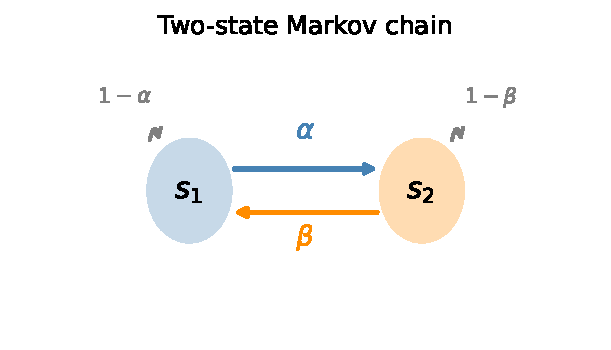
\includegraphics[width=\linewidth]{fig_two_state_chain}
    \end{column}
    \begin{column}{0.45\textwidth}
      \textbf{Two-state chain:}
      $\bfP = \begin{pmatrix}1-\alpha & \alpha \\ \beta & 1-\beta\end{pmatrix}$

      Stationary: $\pi = \left(\tfrac{\beta}{\alpha+\beta},\, \tfrac{\alpha}{\alpha+\beta}\right)$
    \end{column}
  \end{columns}
\end{frame}

\begin{frame}{6.2 Ergodic Theorem and Convergence}
  \begin{block}{Proposition 6.2.2 (Ergodic Theorem)}
    If $\bfP$ is \textbf{regular} (ergodic), then there exists a unique stationary distribution $\pi$ with all entries strictly positive, and
    \[
      \bfP^n \to \bm{\Pi}, \quad \text{as } n \to \infty,
    \]
    where $\bm{\Pi}$ is the matrix with each row equal to $\pi$.
  \end{block}

  \begin{block}{Corollary 6.2.3}
    For any initial distribution $\bfmu$:
    \[
      \bfmu \bfP^n \to \pi \quad \text{as } n \to \infty.
    \]
  \end{block}

  \textbf{Total variation distance:}
  \[
    \dTV(\bfmu, \bfv) = \tfrac{1}{2}\sum_{s \in \mathcal{S}} |\mu_s - v_s|.
  \]

  \textbf{Mixing time:}
  \[
    \tau(\varepsilon) = \min_{n \in \mathbb{N}}\{\dTV(\bfmu\bfP^n,\, \pi) \le \varepsilon\}.
  \]
\end{frame}

\begin{frame}{6.2 Update Function and Detailed Balance}
  \begin{block}{Proposition 6.2.4 (Update Function)}
    Given $\bfP$ and initial distribution $\mu$, there exist functions $\varphi: \mathcal{S} \times [0,1] \to \mathcal{S}$ and $\psi: [0,1] \to \mathcal{S}$ such that
    \[
      X_0 = \psi(U_0), \qquad X_{n+1} = \varphi(X_n, U_{n+1}),
    \]
    where $U_0, U_1, \ldots$ are i.i.d.\ $\mathcal{U}[0,1]$.
  \end{block}

  \begin{block}{Proposition 6.2.5 (Detailed Balance Condition — DBC)}
    If positive weights $(w_s)_{s \in \mathcal{S}}$ satisfy
    \[
      w_s\, p_{ss'} = w_{s'}\, p_{s's}, \qquad \forall\, s, s' \in \mathcal{S},
    \]
    then $\pi_s = w_s / \sum_{s'} w_{s'}$ is a stationary distribution.
  \end{block}

  The DBC is equivalent to \textbf{reversibility}: $(X_0, X_1, \ldots, X_n) \overset{d}{=} (X_n, X_{n-1}, \ldots, X_0)$ when $X_0 \sim \pi$.
\end{frame}

\begin{frame}{6.2 Random Walks on Graphs}
  \begin{block}{Example 6.2.7 (Simple Random Walk on Graph $G$)}
    For a graph $G = (V, E)$, the transition matrix $\bfQ = (q_{vv'})$ is
    \[
      q_{vv'} = \begin{cases} \frac{1}{\deg(v)}, & \text{if } v' \in \mathcal{N}(v), \\ 0, & \text{otherwise.} \end{cases}
    \]
    Setting $w_v = \deg(v)$ satisfies DBC, so the stationary distribution is
    \[
      \pi_v = \frac{\deg(v)}{2|E|}, \quad v \in V.
    \]
  \end{block}

  \textbf{Self-loop modification} (for aperiodicity): with probability $\beta \in (0,1)$, stay at current vertex:
  \[
    q_{vv'} = \begin{cases} \beta, & v=v', \\ \frac{1-\beta}{\deg(v)}, & v' \in \mathcal{N}(v). \end{cases}
  \]
  This does not change the stationary distribution.
\end{frame}

% ============================================================
\section{6.3 Constructing a Markov Chain with Prescribed Stationary Distribution}
% ============================================================

\begin{frame}{6.3 MCMC: The Big Idea}
  \begin{block}{Problem}
    Given a \textbf{target distribution} $\pi$ on a large state space $\mathcal{S} = \{s_1,\ldots,s_N\}$, construct a Markov chain $(Y_n)$ with stationary distribution $\pi$ that is easy to simulate.
  \end{block}

  \textbf{Goals of MCMC:}
  \begin{enumerate}
    \item[\textbf{(A1)}] Sample from a distribution ``close'' to $\pi$ (and in some cases, exactly from $\pi$).
    \item[\textbf{(A2)}] Approximate $\pi(A) = \sum_{s \in A} \pi_s$ for specific subsets $A \subseteq \mathcal{S}$.
  \end{enumerate}

  \medskip
  \textbf{Key insight:} We only need to compute \emph{ratios} $\pi_{s'}/\pi_s$ — the normalizing constant cancels.

  \medskip
  \textbf{Two main approaches:}
  \begin{itemize}
    \item \textbf{Metropolis-Hastings:} propose a move, accept/reject based on ratio.
    \item \textbf{Gibbs sampler:} update one coordinate at a time from its full conditional.
  \end{itemize}
\end{frame}

% ────────────────────────────────────
\subsection{6.3.1 Metropolis and Metropolis-Hastings}
% ────────────────────────────────────

\begin{frame}{6.3.1 Metropolis Algorithm}
  \begin{block}{Setup}
    Let $\bfQ = (q_{ss'})$ be a \textbf{symmetric}, regular transition matrix (the \emph{proposal} matrix).
    Define the acceptance probability:
    \[
      \alpha = \min\!\left(1,\, \frac{\pi_{s'}}{\pi_s}\right).
    \]
  \end{block}

  \begin{columns}[T]
    \begin{column}{0.48\textwidth}
      \textbf{Algorithm 42 (Metropolis):}
      \begin{enumerate}
        \item Current state: $Y_k = s$.
        \item Propose $X \sim \mathbf{q}_s$.
        \item Set $\alpha = \min\!\left(1,\, \pi_X/\pi_s\right)$.
        \item Generate $U \sim \mathcal{U}[0,1]$.
        \item If $U \le \alpha$: $Y_{k+1} = X$.
        \item Else: $Y_{k+1} = Y_k$.
      \end{enumerate}
    \end{column}
    \begin{column}{0.48\textwidth}
      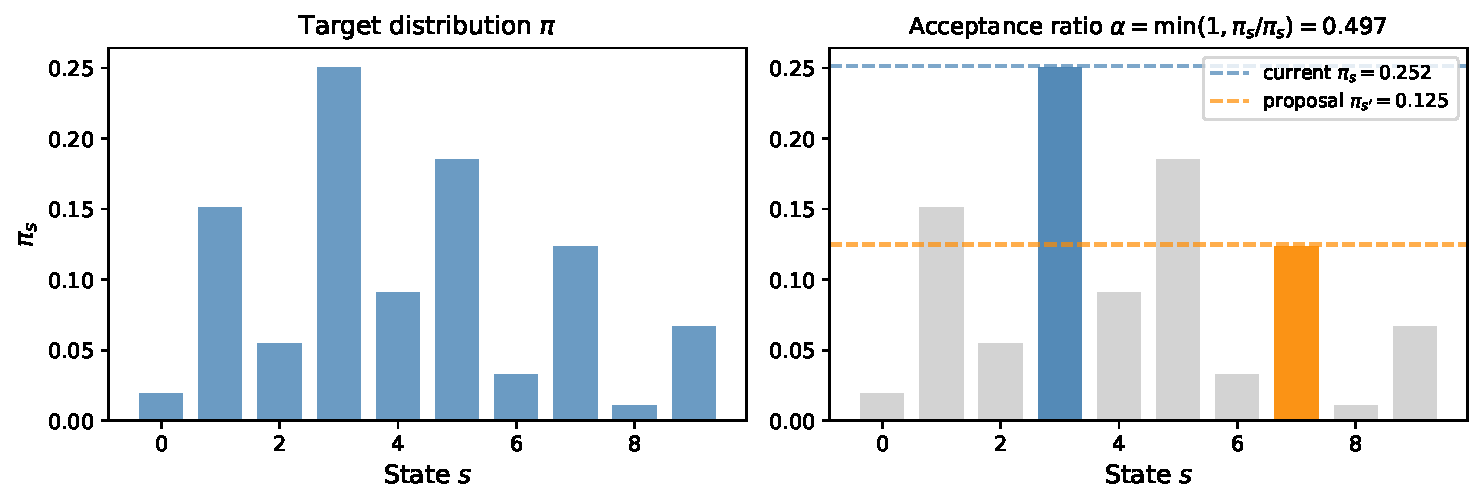
\includegraphics[width=\linewidth]{fig_metropolis_acceptance}
    \end{column}
  \end{columns}

  \begin{block}{Proposition 6.3.1}
    If $\bfQ$ is symmetric and regular, then $\bfP$ is regular with stationary distribution $\pi$.
  \end{block}
\end{frame}

\begin{frame}{6.3.1 Metropolis-Hastings Algorithm}
  \textbf{Extension:} Drop the symmetry assumption on $\bfQ$.

  \begin{block}{Algorithm 43 (Metropolis-Hastings)}
    \begin{enumerate}
      \item Current state: $Y_k = s$.
      \item Propose $X \sim \mathbf{q}_s$.
      \item Set $\alpha = \min\!\left(1,\, \dfrac{\pi_X\, q_{Xs}}{\pi_s\, q_{sX}}\right)$.
      \item If $U \le \alpha$: accept $Y_{k+1} = X$; else $Y_{k+1} = Y_k$.
    \end{enumerate}
  \end{block}

  \begin{block}{Proposition 6.3.2 (Metropolis-Hastings)}
    Let $\bfQ$ be regular with $q_{ss'} > 0 \Leftrightarrow q_{s's} > 0$. Then $\bfP$ with
    \[
      p_{ss'} = q_{ss'}\,\alpha_{ss'}, \quad s \neq s', \qquad
      \alpha_{ss'} = \min\!\left(1,\, \frac{\pi_{s'}\,q_{s's}}{\pi_s\,q_{ss'}}\right),
    \]
    is a regular matrix with stationary distribution $\pi$.
  \end{block}

  \textbf{Key:} Only ratios $\pi_{s'}/\pi_s$ are needed — normalizing constant cancels.
\end{frame}

\begin{frame}[fragile]{6.3.1 Metropolis-Hastings: Python Implementation}
\begin{lstlisting}[style=python]
import numpy as np

def metropolis_hastings(log_pi, proposal, x0, n_steps):
    """
    Generic Metropolis-Hastings sampler.
    log_pi  : callable, log of (unnormalized) target density
    proposal: callable, proposal(x) -> (x_new, log_q_ratio)
              where log_q_ratio = log q(x_new->x) - log q(x->x_new)
    x0      : initial state
    n_steps : number of steps
    """
    samples = [x0]
    x = x0
    n_accept = 0
    for _ in range(n_steps):
        x_new, log_q_ratio = proposal(x)
        # MH acceptance ratio
        log_alpha = (log_pi(x_new) - log_pi(x)) + log_q_ratio
        if np.log(np.random.rand()) < log_alpha:
            x = x_new
            n_accept += 1
        samples.append(x)
    print(f"Acceptance rate: {n_accept/n_steps:.1%}")
    return np.array(samples)

# Example: target = mixture of Gaussians, symmetric random walk proposal
def log_pi_mix(x):
    return np.log(0.4*np.exp(-0.5*(x+2)**2) + 0.6*np.exp(-0.5*(x-3)**2/4))

def rw_proposal(x, sigma=1.5):
    x_new = x + np.random.normal(0, sigma)
    return x_new, 0.0   # symmetric => log_q_ratio = 0

np.random.seed(42)
chain = metropolis_hastings(log_pi_mix, rw_proposal, x0=0.0, n_steps=5000)
I_hat = chain[500:].mean()   # burn-in of 500
print(f"E[X] estimate: {I_hat:.4f}")
\end{lstlisting}
\end{frame}

\begin{frame}{6.3.1 MH Trace and Convergence}
  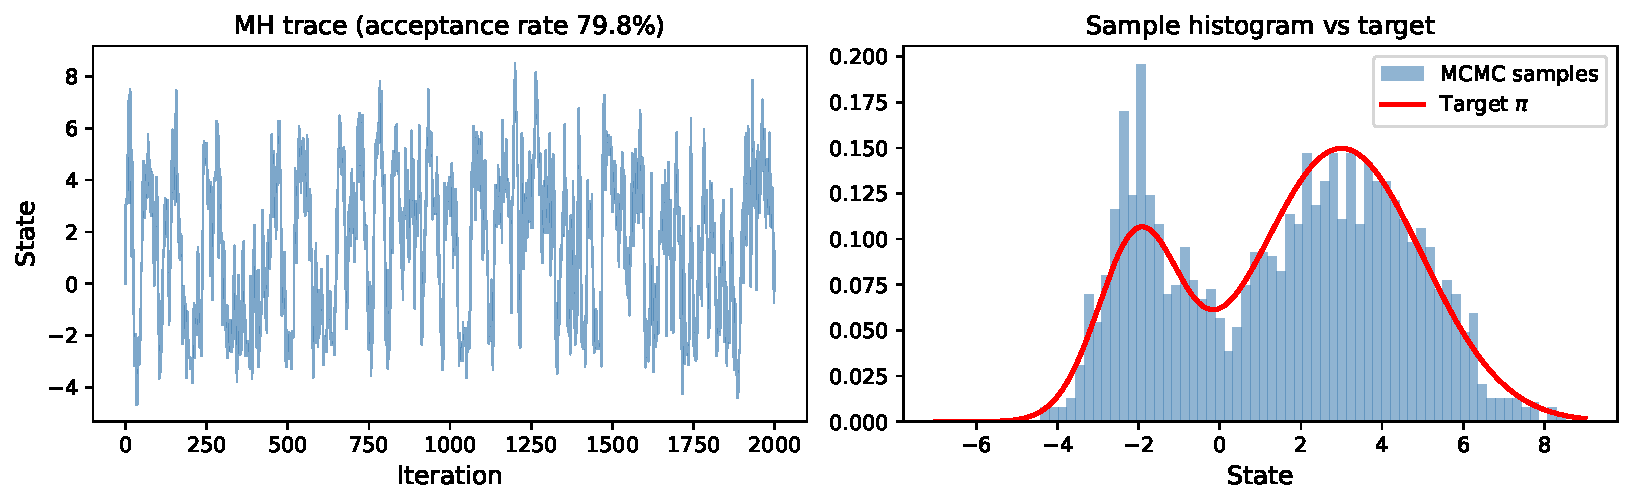
\includegraphics[width=\linewidth]{fig_mh_trace}

  \textbf{Observations:}
  \begin{itemize}
    \item After a \textbf{burn-in} period the chain mixes and samples from $\pi$.
    \item The proposal step size $\sigma$ controls the acceptance rate (target $\approx 20$--$50\%$).
    \item The sample histogram converges to the target density.
  \end{itemize}
\end{frame}

% ────────────────────────────────────
\subsection{6.3.2 Gibbs Sampler}
% ────────────────────────────────────

\begin{frame}{6.3.2 Gibbs Sampler: Setup}
  \textbf{Setting:} State space $\mathcal{S} = C^V$ where $V$ is a set of vertices (e.g.\ graph nodes) and $C = \{1,\ldots,r\}$ is a finite set of values.

  \begin{block}{Full Conditional Distribution}
    For a configuration $\xi \in \mathcal{S}$ and vertex $v \in V$, define
    \[
      p_{\xi,v}(c) = \PP(Z(v) = c \mid Z_{-v} = \xi_{-v}), \quad c \in C,
    \]
    where $Z \sim \pi$ and $\xi_{-v}$ is $\xi$ with the $v$-th component removed.
  \end{block}

  \begin{block}{Gibbs Sampler (one step)}
    \begin{enumerate}
      \item Current configuration: $\xi$.
      \item Pick vertex $v \in V$ uniformly at random.
      \item Sample $c \sim p_{\xi,v}(\cdot)$ (the \textbf{full conditional}).
      \item Set $\xi' = \xi(v, c)$ (replace $\xi_v$ with $c$).
    \end{enumerate}
  \end{block}

  \textbf{Key property:} The Gibbs sampler satisfies DBC and has stationary distribution $\pi$.
\end{frame}

\begin{frame}{6.3.2 Gibbs Sampler: Full Conditional Illustration}
  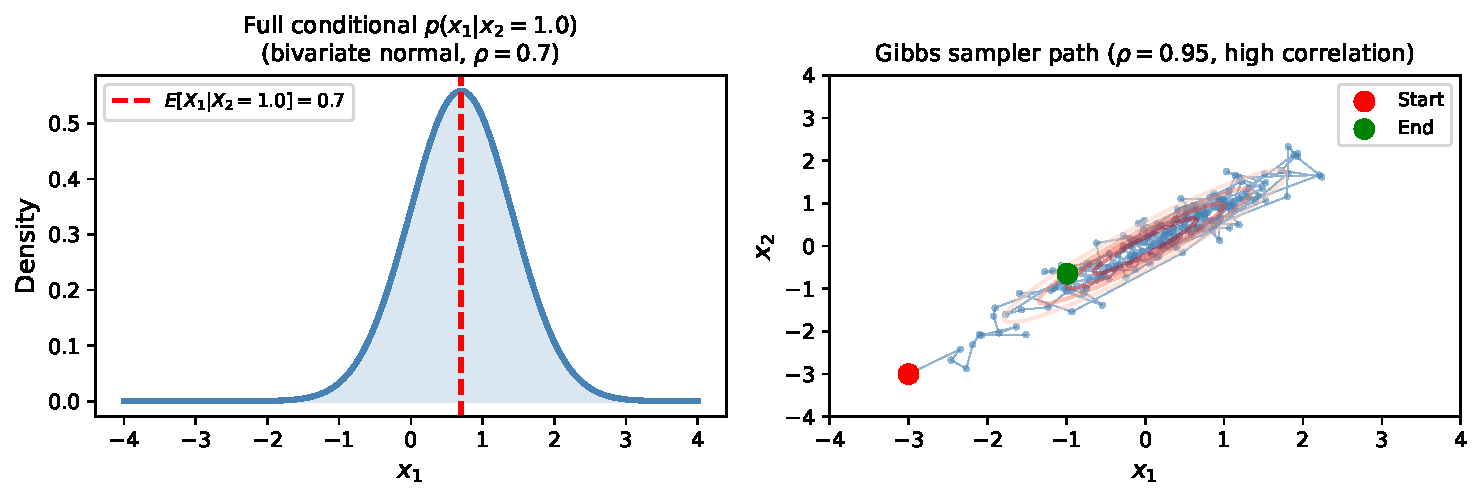
\includegraphics[width=0.95\linewidth]{fig_gibbs_full_conditional}

  \textbf{Left:} Full conditional $p(x_1 | x_2 = 1)$ for a bivariate normal with $\rho = 0.7$.

  \textbf{Right:} Gibbs sampler path for high correlation ($\rho = 0.95$) — characteristic zigzag pattern showing slower mixing than MH.
\end{frame}

\begin{frame}[fragile]{6.3.2 Gibbs Sampler: Python Implementation}
\begin{lstlisting}[style=python]
import numpy as np

def gibbs_sampler(pi_dict, state_space, vertices, n_steps, xi0=None):
    """
    Generic Gibbs sampler on S = C^V.
    pi_dict  : dict mapping configurations (as tuples) to unnormalized probabilities
    vertices : list of vertex labels
    n_steps  : number of Gibbs steps
    """
    import random
    xi = dict(xi0) if xi0 else {v: state_space[0] for v in vertices}
    samples = [tuple(xi[v] for v in vertices)]

    for _ in range(n_steps):
        v = random.choice(vertices)   # pick vertex uniformly
        # Compute full conditional
        weights = []
        for c in state_space:
            xi_test = {**xi, v: c}
            weights.append(pi_dict.get(tuple(xi_test[u] for u in vertices), 0))
        total = sum(weights)
        probs = [w/total for w in weights]
        # Sample from full conditional
        xi[v] = np.random.choice(state_space, p=probs)
        samples.append(tuple(xi[v] for v in vertices))
    return samples

# Example: 2-vertex, 2-color system with Ising-like pi
V = ['v1', 'v2']
C = [0, 1]
beta = 1.0
pi_d = {}
for a in C:
    for b in C:
        pi_d[(a, b)] = np.exp(beta * (a == b))   # prefer same color
chain = gibbs_sampler(pi_d, C, V, n_steps=2000)
print(f"Fraction of (1,1): {sum(s==(1,1) for s in chain)/len(chain):.3f}")
\end{lstlisting}
\end{frame}

% ────────────────────────────────────
\subsubsection{Graph Coloring}
% ────────────────────────────────────

\begin{frame}{6.3.2.1 Graph Coloring with Gibbs Sampler}
  \textbf{Setup:} Graph $G = (V, E)$, $r \ge 2$ colors. A \textbf{proper $r$-coloring} assigns colors from $C = \{1,\ldots,r\}$ to vertices such that no two adjacent vertices share a color.

  \begin{columns}[T]
    \begin{column}{0.48\textwidth}
      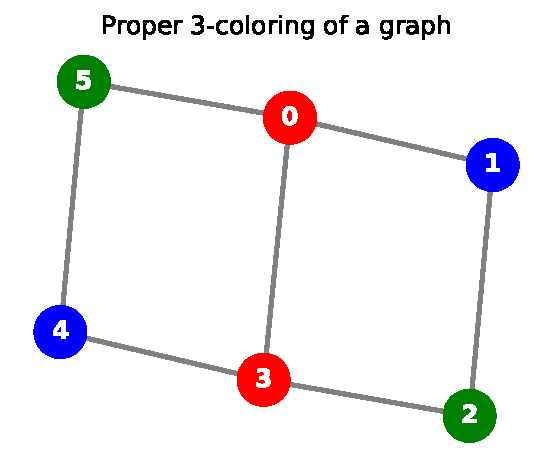
\includegraphics[width=\linewidth]{fig_graph_coloring}
    \end{column}
    \begin{column}{0.48\textwidth}
      \begin{block}{Uniform Distribution on Proper Colorings}
        \[
          \pi_\xi = \frac{1}{z_G}\,\mathbf{1}(\xi \in \Lambda),
        \]
        where $\Lambda$ = set of all proper colorings, $z_G = |\Lambda|$.
      \end{block}
      \textbf{Gibbs step:}
      \begin{enumerate}
        \item Pick $v$ uniformly.
        \item Let $F(v,\xi)$ = colors of $v$'s neighbors.
        \item Pick $c$ uniformly from $C \setminus F(v,\xi)$.
        \item Set $\xi_v \leftarrow c$.
      \end{enumerate}
    \end{column}
  \end{columns}

  \medskip
  \textbf{Theorem (Jerrum '95):} If $r \ge 2\Delta + 1$ (where $\Delta = \max\deg$), the Gibbs sampler is \textbf{rapidly mixing} with $\tau(\kappa) \le \frac{r}{r-2\Delta}|V|\ln(|V|/\kappa)$.
\end{frame}

% ────────────────────────────────────
\subsubsection{Hard-core Model}
% ────────────────────────────────────

\begin{frame}{6.3.2.2 Hard-core Model}
  \textbf{Setup:} Graph $G = (V, E)$, $\lambda > 0$. Each vertex is either \emph{occupied} (1) or \emph{empty} (0). An \textbf{independent set} (hard-core configuration) has no two adjacent vertices occupied.

  \begin{columns}[T]
    \begin{column}{0.5\textwidth}
      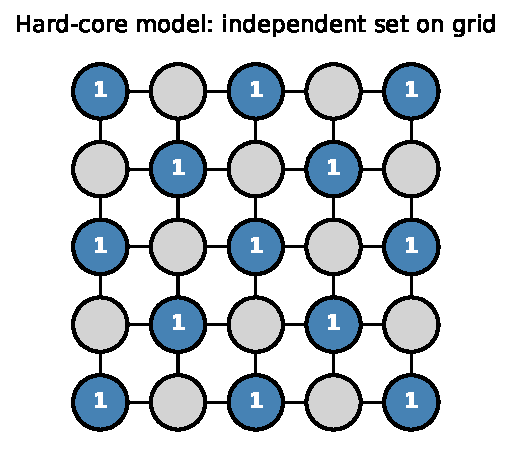
\includegraphics[width=\linewidth]{fig_hardcore_grid}
    \end{column}
    \begin{column}{0.46\textwidth}
      \begin{block}{Hard-core Distribution}
        \[
          \pi_\xi = \frac{\lambda^{\sum_v \xi(v)}}{z_\lambda}\,\mathbf{1}(\xi \in \Lambda),
        \]
        $\Lambda$ = all independent sets.
      \end{block}
      \textbf{Full conditional} (Eq.~6.3.13):
      \[
        p_{\xi,v}(1) = \frac{\lambda}{1+\lambda}\,\mathbf{1}(\text{all nbrs = 0})
      \]
    \end{column}
  \end{columns}

  \bigskip
  The Gibbs sampler for the hard-core model (Algorithm 47 in the book) samples from the hard-core distribution by updating one vertex at a time, accepting occupation with probability $\lambda/(1+\lambda)$ if all neighbors are unoccupied.
\end{frame}

% ────────────────────────────────────
\subsubsection{Ising Model}
% ────────────────────────────────────

\begin{frame}{6.3.2.4 Ising Model}
  \textbf{Setup:} Graph $G = (V, E)$, $\beta \in \mathbb{R}$. Each vertex has spin $\xi(v) \in \{-1, +1\}$.

  \begin{block}{Ising Distribution}
    \[
      \pi_\xi = \frac{1}{z(\beta)}\exp\!\left(\beta \sum_{\{u,v\} \in E} \xi(u)\,\xi(v)\right).
    \]
    \begin{itemize}
      \item $\beta > 0$: ferromagnet (spins align with neighbors).
      \item $\beta < 0$: anti-ferromagnet (spins oppose neighbors).
    \end{itemize}
  \end{block}

  \begin{columns}[T]
    \begin{column}{0.48\textwidth}
      \textbf{Gibbs update function:}
      \[
        \varphi(\xi, v, u) = \begin{cases}
          \xi(v \to -1) & \text{if } u \in [0,\alpha(\xi,v)), \\
          \xi(v \to +1) & \text{if } u \in [\alpha(\xi,v), 1],
        \end{cases}
      \]
      where $\alpha(\xi, v) = \PP(Z(v) = -1 \mid Z_{-v} = \xi_{-v})$.
    \end{column}
    \begin{column}{0.48\textwidth}
      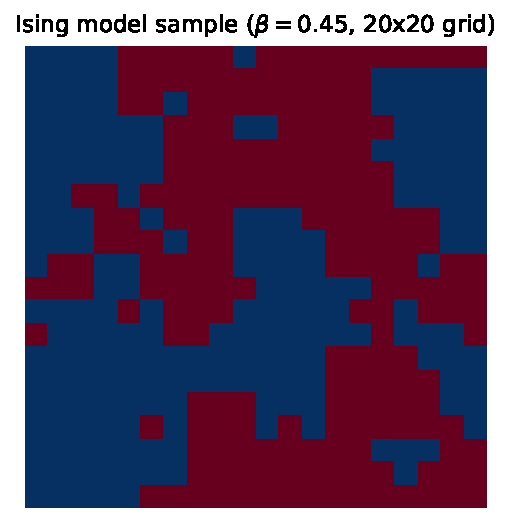
\includegraphics[width=\linewidth]{fig_ising_sample}
    \end{column}
  \end{columns}
\end{frame}

\begin{frame}[fragile]{6.3.2.4 Ising Model: Python Implementation}
\begin{lstlisting}[style=python]
import numpy as np

def ising_gibbs(n, beta, n_steps=50000, seed=0):
    """Gibbs sampler for Ising model on n x n periodic grid."""
    np.random.seed(seed)
    config = np.random.choice([-1, 1], size=(n, n))

    for step in range(n_steps):
        i, j = np.random.randint(0, n, 2)
        # Sum of neighboring spins (periodic boundary)
        nbr_sum = (config[(i-1)%n, j] + config[(i+1)%n, j] +
                   config[i, (j-1)%n] + config[i, (j+1)%n])
        # Full conditional: P(spin = +1 | neighbors)
        h = beta * nbr_sum
        prob_plus = np.exp(h) / (np.exp(h) + np.exp(-h))
        config[i, j] = 1 if np.random.rand() < prob_plus else -1

    return config

# Run for beta = 0.44 (near critical temperature for 2D Ising)
config = ising_gibbs(n=20, beta=0.44, n_steps=100000)
magnetization = config.mean()
print(f"Magnetization: {magnetization:.4f}")
\end{lstlisting}

\medskip
\textbf{Critical temperature} for 2D Ising: $\beta_c = \frac{1}{2}\ln(1+\sqrt{2}) \approx 0.4407$.
\end{frame}

% ============================================================
\section{6.4 Perfect Simulation: Sampling Exactly from $\pi$}
% ============================================================

\begin{frame}{6.4 Perfect Simulation: Motivation}
  \textbf{Problem with standard MCMC:} The chain $(X_n)$ only \emph{approximates} $\pi$ — we never sample exactly from $\pi$.

  \medskip
  \begin{block}{Perfect Simulation}
    Generate a sample \textbf{exactly} from $\pi$ in finite (random) time, without knowing when the chain has mixed.
  \end{block}

  \textbf{Key idea:} \textbf{Coupling from the Past (CFTP)} — run the chain \emph{backwards} in time from $-\infty$ to $0$, starting from \textbf{all} possible initial states simultaneously, and detect when they all coalesce.

  \bigskip
  \textbf{Requires:}
  \begin{itemize}
    \item A \textbf{monotone} update function $\varphi$ (for efficient implementation).
    \item The ability to track only the \textbf{minimum} and \textbf{maximum} configurations.
  \end{itemize}
\end{frame}

% ────────────────────────────────────
\subsection{6.4.1 CFTP Algorithm}
% ────────────────────────────────────

\begin{frame}[allowframebreaks]{6.4.1 Coupling from the Past (CFTP)}
  \textbf{State space:} $\mathcal{S} = C^V$ with partial order $\preceq$ and update function $\varphi$.

  \begin{block}{Algorithm 50 (CFTP for Monotone Systems)}
    \textbf{Require:} State space $\mathcal{S} = C^V$, monotone $\pi$.
    \begin{enumerate}
      \item Set $n = 1$.
      \item Start a bivariate chain $Y_k^{-N_n} = (X_k^{\xi_{\min},-N_n},\, X_k^{\xi_{\max},-N_n})$ at time $-N_n$ from $(\xi_{\min}, \xi_{\max})$.
            Run using the \textbf{same} i.i.d.\ $U_i$ random variables.
      \item \textbf{If} at time $0$ we have $Y_0^{-N_n} = (\xi, \xi)$: \textbf{return} $\xi$ and \textbf{stop}.
      \item \textbf{Else} set $n = n+1$ and go to Step 2 (reuse previously generated $U_i$).
    \end{enumerate}
  \end{block}

  \begin{block}{Theorem 6.4.2}
    \begin{enumerate}[(i)]
      \item Algorithm 50 terminates with probability 1.
      \item The output $\xi$ has distribution exactly $\pi$.
    \end{enumerate}
  \end{block}

  \framebreak

  \textbf{Key CFTP property (coupling inequality):}
  \[
    \dTV(\pi, \pi') \le \PP(Y_0^{-N_n} \ne Y_0^{\tau_{\rm cftp}}) \le \PP(\tau_{\rm cftp} < -N_n) \le \varepsilon.
  \]

  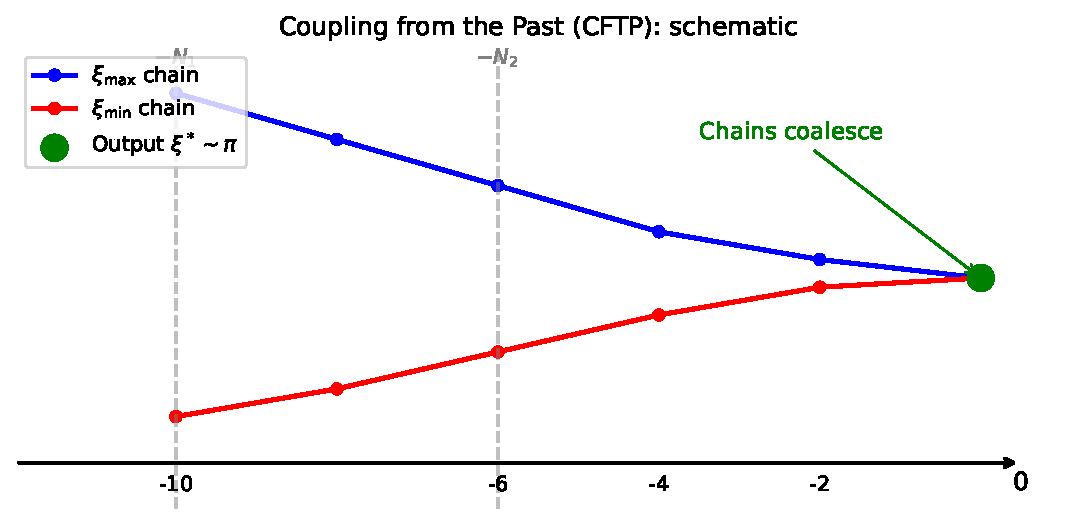
\includegraphics[width=0.9\linewidth]{fig_cftp_schematic}

  \textbf{Intuition:}
  \begin{itemize}
    \item Two chains (from $\xi_{\min}$ and $\xi_{\max}$) coalesce because the update function is \textbf{monotone}: $\xi \preceq \xi' \Rightarrow \varphi(\xi, v, u) \preceq \varphi(\xi', v, u)$.
    \item Only need to track the min/max chains — all others lie between them.
  \end{itemize}
\end{frame}

\begin{frame}{6.4.2 Theory of CFTP}
  \begin{block}{Definition: Monotone Markov Chain (Def.\ 6.4.5)}
    A Markov chain with update function $\varphi$ is \textbf{monotone} w.r.t.\ $\preceq$ if
    \[
      \xi \preceq \xi' \Rightarrow \varphi(\xi, v, u) \preceq \varphi(\xi', v, u) \quad \forall\, v \in V,\, u \in [0,1].
    \]
  \end{block}

  \begin{block}{Definition: Anti-monotone Chain (Def.\ 6.4.11)}
    The chain is \textbf{anti-monotone} if
    \[
      \xi \preceq \xi' \Rightarrow \varphi(\xi', v, u) \preceq \varphi(\xi, v, u) \quad \forall\, v,u.
    \]
  \end{block}

  \textbf{Examples:}
  \begin{itemize}
    \item \textbf{Hard-core model} ($\lambda > 0$): monotone chain — higher occupation encourages more occupation.
    \item \textbf{Ferromagnet Ising} ($\beta > 0$): monotone chain.
    \item \textbf{Anti-ferromagnet Ising} ($\beta < 0$): anti-monotone chain — alternating update handles this.
  \end{itemize}
\end{frame}

\begin{frame}[fragile]{6.4.1 CFTP: Python Sketch (Hard-core Model)}
\begin{lstlisting}[style=python]
import numpy as np

def cftp_hardcore(G, lam, max_attempts=20):
    """
    CFTP for hard-core model on graph G with parameter lambda.
    G : dict {vertex: [neighbors]}
    """
    vertices = list(G.keys())
    n = len(vertices)

    for attempt in range(max_attempts):
        N = 2 ** attempt           # doubling strategy
        # Pre-generate uniform random variables U[i], V[i]
        Us = np.random.rand(N)
        Vs = np.random.randint(0, n, N)

        # Track min (all 0) and max (all 1 feasible)
        xi_min = {v: 0 for v in vertices}
        xi_max = {v: 1 for v in vertices}

        for k in range(N):
            v = vertices[Vs[k]]
            u = Us[k]
            # Update xi_min
            nbrs_min = any(xi_min[w] == 1 for w in G[v])
            xi_min[v] = 0 if nbrs_min else (1 if u < lam/(1+lam) else 0)
            # Update xi_max
            nbrs_max = any(xi_max[w] == 1 for w in G[v])
            xi_max[v] = 0 if nbrs_max else (1 if u < lam/(1+lam) else 0)

        if xi_min == xi_max:
            return xi_min   # exact sample from pi
    return xi_min            # fallback

# Example: path graph on 5 vertices
G_path = {0:[1], 1:[0,2], 2:[1,3], 3:[2,4], 4:[3]}
sample = cftp_hardcore(G_path, lam=2.0)
print(f"CFTP sample: {sample}")
\end{lstlisting}
\end{frame}

\begin{frame}{6.4.4 Anti-ferromagnet Ising Model}
  \begin{block}{Anti-ferromagnet Ising: $\beta < 0$}
    The update function:
    \[
      \varphi(\xi, v, u) = \begin{cases}
        \xi(v \to -1) & \text{if } u \in [0, \alpha(\xi, v)), \\
        \xi(v \to +1) & \text{if } u \in [\alpha(\xi,v), 1].
      \end{cases}
    \]
    For $\beta < 0$: $0 < \alpha(\xi, v) < 1$, and the chain is \textbf{anti-monotone}.
  \end{block}

  \begin{block}{Algorithm 52 (CFTP for Anti-ferromagnet Ising)}
    \textbf{Require:} Graph $G = (V, E)$, parameter $\beta < 0$.
    \begin{enumerate}
      \item Start bivariate chain $Y_{-N_n}^{-N_n} = (\xi_{\min}, \xi_{\max})$ where $\xi_{\min}$ assigns $-1$ to all vertices and $\xi_{\max}$ assigns $+1$ to all.
      \item Run using \textbf{same} $U_k$, $W_k$ (vertex selector).
      \item The bivariate update interchanges the roles of the two chains when updating, exploiting anti-monotonicity.
      \item Stop when coalescence is detected.
    \end{enumerate}
  \end{block}

  \textbf{Proposition 6.4.17:} Algorithm 51 terminates with probability 1 and its output has distribution $\pi$.
\end{frame}

% ============================================================
\section{6.5 Approximate Counting}
% ============================================================

\begin{frame}[allowframebreaks]{6.5 Approximate Counting: Introduction}
  \textbf{Question:} How many proper colorings does a graph have? How many independent sets?

  \begin{block}{Counting Problem}
    Given a graph $G = (V, E)$ and value set $C = \{1,\ldots,r\}$, let
    \[
      z_G = |\Lambda|, \quad \Lambda \subseteq C^V \text{ = set of feasible configurations}.
    \]
    Computing $z_G$ \textbf{exactly} is \#P-complete in general.
  \end{block}

  \begin{block}{$(\varepsilon, \delta)$-Approximation Scheme}
    An estimator $\hat{z}_G$ is an \textbf{$(\varepsilon, \delta)$-approximation scheme} (FPRASC) for $z_G$ if
    \[
      \PP\bigl(|\hat{z}_G - z_G| > \varepsilon\, z_G\bigr) \le \delta,
    \]
    with running time polynomial in $1/\varepsilon$, $\ln(1/\delta)$, and problem size.
  \end{block}

  \framebreak

  \textbf{Naïve estimator:} Sample $R$ random subsets of $V$, check if independent. With $p = z_G/2^M$,
  \[
    \hat{z}_G^{\rm naive} = 2^M \hat{Y}_R, \quad \mathbb{E}\hat{Y}_R = z_G/2^M.
  \]
  \textbf{Problem:} $p$ may be exponentially small, requiring exponentially many samples.

  \medskip
  \textbf{Solution (telescoping):} Decompose
  \[
    z_G = z_0 \times \frac{z_1}{z_0} \times \frac{z_2}{z_1} \times \cdots \times \frac{z_m}{z_{m-1}},
  \]
  where each ratio $\varrho_i = z_i/z_{i-1} \ge 1/2$ is efficiently estimable.

  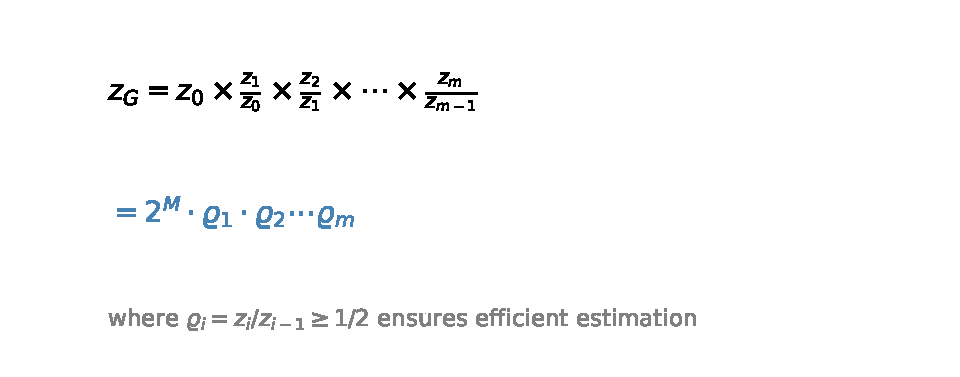
\includegraphics[width=0.7\linewidth]{fig_fpras_decomposition}
\end{frame}

% ────────────────────────────────────
\subsection{6.5.1 Independent Sets — FPRAS}
% ────────────────────────────────────

\begin{frame}[allowframebreaks]{6.5.1 Independent Sets: FPRAS}
  \textbf{Setup:} $G = (V, E)$, $M = |V|$, $m = |E|$. Let $G_i = (V, E_i)$ where $E_i = \{e_1,\ldots,e_i\}$.
  Let $z_i = |\Lambda_{G_i}|$ (number of independent sets of $G_i$), and $z_0 = 2^M$.

  \begin{block}{Key Lemma 6.5.7}
    $\varrho_i = z_i/z_{i-1} \ge 1/2$ for all $i$.
  \end{block}
  \textit{Proof sketch:} Adding edge $(w,v)$ removes independent sets containing both $w$ and $v$; at most half of all independent sets of $G_{i-1}$ contain both endpoints.

  \begin{block}{Proposition 6.5.4 (FPRAS for $z_G$)}
    Let $(X_n)$ be rapidly mixing with stationary distribution $\pi^{(i)}_\xi = \mathbf{1}(\xi \in \Lambda_{G_i})/z_i$ and mixing time $\tau(\kappa)$. Then there exists an $(\varepsilon, \delta)$-FPRASC for $z_G$ with running time
    \[
      \frac{200m^3}{\varepsilon^2}\ln\!\left(\frac{2m}{\delta}\right)\tau\!\left(\frac{\varepsilon}{16m}\right).
    \]
  \end{block}

  \framebreak

  \begin{block}{Algorithm 54: $(\varepsilon/2m, \delta/m)$-FPRASC for $\varrho_i$}
    \textbf{Require:} Graphs $G_{i-1}$, $G_i$; parameters $\delta, \varepsilon, m$; rapidly mixing chain $(X_n^{(i)})$.
    \begin{enumerate}
      \item For $j = 1$ to $R = \frac{200m^2}{\varepsilon^2}\ln\!\left(\frac{2m}{\delta}\right)$:
      \begin{itemize}
        \item Generate approximate sample $\xi$ from $\pi^{(i-1)}$ (run chain for $\tau(\varepsilon/(16m))$ steps).
        \item Set $\tilde{Y}_j^{(i)} = 1$ if $\xi \in \Lambda_{G_i}$, else $0$.
      \end{itemize}
      \item Return $\tilde{\varrho}_i = \frac{1}{R}\sum_{j=1}^R \tilde{Y}_j^{(i)}$.
    \end{enumerate}
  \end{block}

  \begin{block}{Algorithm 55: $(\varepsilon, \delta)$-FPRASC for $z_G$}
    \begin{enumerate}
      \item For $i = 1$ to $m$: estimate $\varrho_i$ via Algorithm 54.
      \item Return $\hat{z}_G = 2^M \prod_{i=1}^m \tilde{\varrho}_i$.
    \end{enumerate}
  \end{block}
\end{frame}

% ────────────────────────────────────
\subsection{6.5.2 Graph Colorings and Knapsack}
% ────────────────────────────────────

\begin{frame}[allowframebreaks]{6.5.2 Graph Colorings and Knapsack FPRAS}
  \textbf{Generalized framework (Proposition 6.5.13):} Apply the same telescoping idea to any counting problem admitting:
  \begin{enumerate}
    \item A sequence $\Lambda_0, \Lambda_1, \ldots, \Lambda_t \equiv \Lambda$ with $t$ polynomial in $|G|$ and $z_0$ known.
    \item Rapidly mixing chains with uniform stationary distribution on $\Lambda_i$ and mixing time $\tau(\kappa)$.
    \item $\varrho_i := z_i/z_{i-1} \ge 1/2$.
  \end{enumerate}
  Running time: $\frac{200t^3}{\varepsilon^2}\ln\!\left(\frac{2t}{\delta}\right)\tau\!\left(\frac{\varepsilon}{16t}\right)$.

  \framebreak

  \textbf{Graph colorings:}
  \begin{block}{Lemma 6.5.14}
    If $r > 2\Delta^2$, then $\varrho_i \ge 1/2$.
  \end{block}

  \begin{block}{Lemma 6.5.16}
    If $r > 2\Delta^2$, there exists an $(\varepsilon, \delta)$-FPRASC for the number of proper colorings with running time $O\!\left(\frac{m^3}{\varepsilon^2}\ln\!\left(\frac{2m}{\delta}\right)\frac{r}{r-2\Delta}M\ln\!\left(\frac{16mM}{\varepsilon}\right)\right)$.
  \end{block}

  \textbf{Knapsack:}
  \begin{block}{Lemma 6.5.18 (Dyer \emph{et al.}\ [156])}
    The Gibbs sampler for 0-1 knapsack (Algorithm 57) is rapidly mixing with mixing time
    \[
      \tau(\kappa) = O(d^{9/2+\kappa}).
    \]
  \end{block}
  This gives an $(\varepsilon,\delta)$-FPRASC for the number of knapsack solutions with running time $O(d^{15/2+\varepsilon/(16d)}/\varepsilon^2 \cdot \ln(2d/\delta))$.
\end{frame}

\begin{frame}[fragile]{6.5 Approximate Counting: Python Sketch}
\begin{lstlisting}[style=python]
import numpy as np

def count_independent_sets_fpras(G, eps=0.1, delta=0.05, tau_func=None):
    """
    FPRASC for number of independent sets using edge-by-edge telescoping.
    G        : list of edges [(u,v), ...]
    eps, delta: accuracy parameters
    tau_func : mixing time function (use constant for demo)
    """
    vertices = list(set(v for e in G for v in e))
    M = len(vertices)
    m = len(G)
    z0 = 2 ** M

    R = int(200 * m**2 / eps**2 * np.log(2*m/delta)) + 1
    tau = tau_func(eps/(16*m)) if tau_func else 100  # mixing steps

    rho_estimates = []
    current_edges = []
    for edge in G:
        # Estimate rho_i = z_i / z_{i-1}
        count_feasible = 0
        for _ in range(R):
            # Sample from pi^{(i-1)} via Gibbs (simplified)
            xi = {v: np.random.randint(2) for v in vertices}
            # Check if xi is feasible for G_i (with new edge)
            new_u, new_v = edge
            feasible_new = not (xi.get(new_u, 0) == 1 and xi.get(new_v, 0) == 1)
            count_feasible += feasible_new
        rho_i = count_feasible / R
        rho_estimates.append(max(rho_i, 1e-10))
        current_edges.append(edge)

    import math
    z_hat = z0 * math.prod(rho_estimates)
    return z_hat, rho_estimates

# Small example: triangle graph
G_triangle = [(0,1), (1,2), (0,2)]
z_hat, rhos = count_independent_sets_fpras(G_triangle, eps=0.2, delta=0.1)
print(f"Estimated z_G = {z_hat:.1f}  (true = 4 for triangle)")
\end{lstlisting}
\end{frame}

% ============================================================
\section{6.6 Computational Biology: Motif Finding}
% ============================================================

\begin{frame}[allowframebreaks]{6.6 Motif Finding Problem}
  \textbf{Biological context:} Identify conserved sequence patterns (motifs) in DNA/protein sequences.

  \begin{block}{Setup}
    \begin{itemize}
      \item $k$ sequences, each of length $n$, over alphabet $\Sigma = \{A, C, G, T\}$ (or $d = |\Sigma|$).
      \item A \textbf{motif} is a segment of length $w$ injected into each row at a starting position $\xi_i^\bullet \in \{1,\ldots,n-w+1\}$.
      \item \textbf{Background} letters are i.i.d.\ with distribution $\boldsymbol{\theta}_0 = (\theta_{1,0},\ldots,\theta_{d,0})^T$.
      \item \textbf{Motif} letters at position $j$ have distribution $\boldsymbol{\theta}_j = (\theta_{1,j},\ldots,\theta_{d,j})^T$.
      \item The \textbf{position weight matrix} (PWM) is $\boldsymbol{\Theta} = (\boldsymbol{\theta}_1,\ldots,\boldsymbol{\theta}_w)$.
    \end{itemize}
  \end{block}

  \begin{block}{Problem 2}
    Given sequences $\mathbf{R} = (r_{ij})$, $1 \le i \le k$, $1 \le j \le n$, and parameters $\boldsymbol{\theta}_j$ ($j=0,\ldots,w$), find the starting positions $\xi^\bullet = (\xi_1^\bullet,\ldots,\xi_k^\bullet)$.
  \end{block}

  \framebreak

  \textbf{Likelihood function:} For configuration $\xi$, define
  \begin{itemize}
    \item Matrix $\mathbf{A}_\xi$: $k \times w$ matrix, row $i$ = segment of $\mathbf{R}$ starting at $\xi_i$.
    \item Matrix $\mathbf{C}_\xi$: $d \times w$ count matrix, $\mathbf{C}_\xi(i,j) = \#\{l : \mathbf{A}_\xi(l,j) = i\}$.
  \end{itemize}
  The complete-data likelihood is
  \[
    f(\xi) = h(\xi) \times g(\xi) = \prod_{i=1}^d \theta_{i,0}^{\mathbf{D}_\xi(i)} \times \prod_{j=1}^w \prod_{i=1}^d \theta_{i,j}^{\mathbf{C}_\xi(i,j)}.
  \]

  \textbf{Energy of configuration:}
  \[
    H(\xi) = -\log f(\xi).
  \]

  \textbf{Gibbs distribution:}
  \[
    \pi_\xi = \frac{1}{z(T)}\exp\!\left(\frac{1}{T}\log f(\xi)\right) = \frac{f(\xi)^{1/T}}{z(T)}.
  \]
  For small $T$, $\pi$ concentrates on low-energy (high-likelihood) configurations $\xi^\bullet$.
\end{frame}

\begin{frame}{6.6 Gibbs Sampler for Motif Finding}
  \begin{block}{Gibbs Update (Algorithm 58)}
    \begin{enumerate}
      \item Current configuration: $\xi = (\xi_1,\ldots,\xi_k)$.
      \item Pick row $v \in \{1,\ldots,k\}$ uniformly at random.
      \item Compute $\mathbf{A}_\xi$, $\mathbf{C}_\xi$, $\mathbf{R}_{[\xi]^c}$ (background rows excl.\ row $v$).
      \item For each $c = 1,\ldots,n-w+1$, compute
            \[
              p(c) = \frac{\pi_{\xi(v,c)}}{\sum_{r=1}^{n-w+1} \pi_{\xi(v,r)}}.
            \]
      \item Sample $c \sim p(\cdot)$; set $X_{t+1} = \xi(v, c)$.
    \end{enumerate}
  \end{block}

  \begin{columns}[T]
    \begin{column}{0.5\textwidth}
      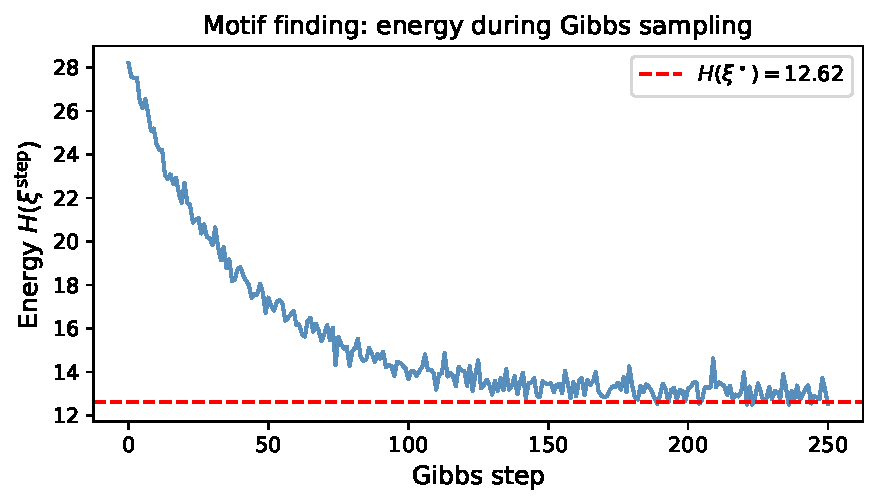
\includegraphics[width=\linewidth]{fig_motif_energy}
    \end{column}
    \begin{column}{0.46\textwidth}
      \textbf{Numerical example (Sect.\ 6.6.3):}
      \begin{itemize}
        \item $k=30$ sequences, $n=20$, $w=13$.
        \item True positions $\xi^\bullet$ simulated.
        \item $H(\xi^\bullet) = 12.62$.
        \item After 200 steps: $H(\xi^{200}) = 12.64$.
        \item Only 2 rows differ from $\xi^\bullet$ by 1 position.
      \end{itemize}
    \end{column}
  \end{columns}
\end{frame}

\begin{frame}[fragile]{6.6 Motif Finding: Python Implementation}
\begin{lstlisting}[style=python]
import numpy as np

def motif_gibbs(R, theta0, Theta, w, T=1.0, n_steps=200, seed=42):
    """
    Gibbs sampler for motif finding (Problem 2).
    R     : (k, n) integer matrix of observed sequences (0-indexed alphabet)
    theta0: background freq vector (length d)
    Theta : (d, w) position weight matrix
    T     : temperature parameter
    """
    np.random.seed(seed)
    k, n = R.shape
    d = len(theta0)
    L = n - w + 1    # number of possible start positions

    def log_f(xi):
        log_lik = 0.0
        for i in range(k):
            s = xi[i]
            motif_part = R[i, s:s+w]
            for j, letter in enumerate(motif_part):
                log_lik += np.log(Theta[letter, j] + 1e-15)
        return log_lik / T

    xi = np.random.randint(0, L, k)    # initial configuration
    H_trace = []

    for step in range(n_steps):
        v = np.random.randint(k)       # pick row uniformly
        log_probs = np.array([
            log_f({**dict(enumerate(xi)), v: c}) for c in range(L)
        ])
        log_probs -= log_probs.max()   # numerical stability
        probs = np.exp(log_probs)
        probs /= probs.sum()
        xi[v] = np.random.choice(L, p=probs)
        H_trace.append(-log_f(xi) * T)
    return xi, H_trace

# Quick demo
np.random.seed(0)
k, n, w, d = 10, 15, 5, 4
R_demo = np.random.randint(0, d, (k, n))
theta0 = np.ones(d)/d
Theta = np.eye(d)[:, :w] * 0.7 + 0.1  # simplified PWM
xi_out, H_trace = motif_gibbs(R_demo, theta0, Theta, w, n_steps=100)
print(f"Final energy: {H_trace[-1]:.2f}")
\end{lstlisting}
\end{frame}

% ============================================================
\section{6.7 Estimating $I = \mathbb{E}f(X)$, $X \sim \pi$}
% ============================================================

\begin{frame}{6.7 Estimating $I = \mathbb{E}f(X)$: Setup}
  \textbf{Goal:} Estimate
  \[
    I = \mathbb{E}f(X) = \sum_{s \in \mathcal{S}} f(s)\,\pi_s,
  \]
  where $X \sim \pi$ and $\pi$ is the stationary distribution of an ergodic Markov chain $(X_n)$.

  \begin{block}{MCMC Estimator}
    Run chain for $R$ steps and use
    \[
      \hat{Y}_R = \frac{1}{R}\sum_{j=1}^R f(X_j).
    \]
  \end{block}

  \textbf{Properties:}
  \begin{itemize}
    \item \textbf{Not unbiased} if $X_0 \not\sim \pi$ (bias $= \beta/R + o(1/R)$).
    \item \textbf{Strongly consistent:} $\hat{Y}_R \to I$ a.s.\ as $R \to \infty$.
    \item \textbf{Asymptotically normal:} $\sqrt{R}(\hat{Y}_R - I) \xrightarrow{d} \mathcal{N}(0, \varsigma^2)$.
  \end{itemize}
\end{frame}

% ────────────────────────────────────
\subsection{6.7.1 Ergodic Theorem and CLT}
% ────────────────────────────────────

\begin{frame}[allowframebreaks]{6.7.1 Ergodic Theorem and CLT for Markov Chains}
  \begin{block}{Proposition 6.7.1 (Strong Law / Ergodic Theorem)}
    If $(X_n)$ is an ergodic finite Markov chain and $f$ is any real-valued function, then
    \[
      \hat{Y}_R = \frac{1}{R}\sum_{j=1}^R f(X_j) \xrightarrow{R\to\infty} I = \sum_{s \in \mathcal{S}} \pi_s f(s) \quad \text{a.s.}
    \]
  \end{block}

  \begin{block}{Proposition 6.7.5 (CLT for Markov Chains)}
    If $(X_n)$ is an ergodic finite Markov chain and $f$ is real-valued, then
    \[
      \sqrt{R}\,(\hat{Y}_R - I) \xrightarrow{d} \mathcal{N}(0, \varsigma^2),
    \]
    where the \textbf{asymptotic variance} (TAVC) satisfies
    \[
      0 < \varsigma^2 = \lim_{R\to\infty} R\,\mathrm{Var}\hat{Y}_R < \infty.
    \]
    The limits are independent of the initial distribution $\mu$.
  \end{block}

  \framebreak

  \textbf{Regenerative structure:} States of the chain returns to $s_0$ at times $\gamma_0, \gamma_1, \ldots$.
  Cycle lengths $\eta_l = \gamma_l - \gamma_{l-1}$ and cycle sums $W_l = \sum_{j=\gamma_{l-1}}^{\gamma_l - 1} f(X_j)$ are i.i.d.

  \[
    I = \lim_{R\to\infty}\hat{Y}_R = \frac{\mathbb{E}W_1}{\mathbb{E}\eta_1} \quad \text{(ratio of i.i.d.\ means)}.
  \]

  \textbf{Asymptotic variance formula:}
  \[
    \varsigma^2 = \frac{\mathrm{Var}(W_1 - I\eta_1)}{\mathbb{E}\eta_1}.
  \]

  \textbf{Via fundamental matrix:} Let $\mathbf{Z} = \mathbf{I} + \sum_{k=1}^\infty (\mathbf{P}^k - \bm{\Pi}) = (\mathbf{I} - (\mathbf{P} - \bm{\Pi}))^{-1}$. Then
  \[
    \varsigma^2 = \rho_0 + 2\sum_{k=1}^\infty \rho_k = \mathrm{Var}Y\!\left(1 + 2\sum_{k=1}^\infty \rho_k\right),
  \]
  and by Lemma 6.7.11:
  \[
    \varsigma^2 = \rho_0 + 2\pi\,\mathrm{diag}(\mathbf{f})(\mathbf{Z}-\mathbf{I})\mathbf{f}^T.
  \]

  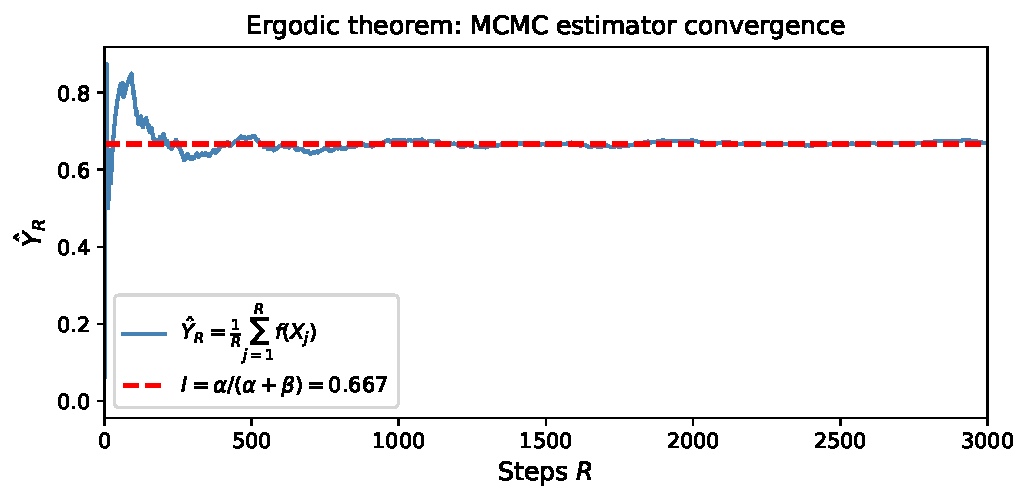
\includegraphics[width=0.85\linewidth]{fig_ergodic_convergence}
\end{frame}

\begin{frame}{6.7 Two-State Chain: Exact Asymptotic Variance}
  \begin{block}{Example 6.7.12}
    Two-state chain $\mathcal{S} = \{0, 1\}$ with $\mathbf{P} = \begin{pmatrix}1-\alpha & \alpha \\ \beta & 1-\beta\end{pmatrix}$, $f(x) = x$.

    \textbf{True value:} $I = \alpha/(\alpha+\beta)$.

    \textbf{Asymptotic variance:}
    \[
      \varsigma^2 = \frac{\alpha\beta(2-\alpha-\beta)}{(\alpha+\beta)^3}.
    \]

    \textbf{Comparison with i.i.d.:} $\mathrm{Var}(Y^{\rm ind}) = \alpha\beta/(\alpha+\beta)^2$, so
    \[
      \frac{\varsigma^2}{\mathrm{Var}(Y^{\rm ind})} = \frac{2-\alpha-\beta}{\alpha+\beta}.
    \]
    MC is better than i.i.d.\ when $\alpha + \beta > 1$.
  \end{block}

  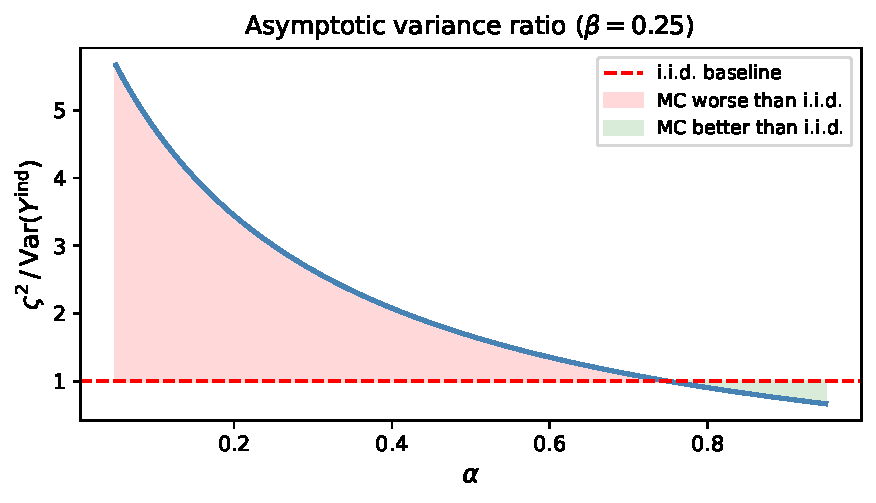
\includegraphics[width=0.7\linewidth]{fig_asymptotic_variance}
\end{frame}

\begin{frame}{6.7 Variance Estimation and Confidence Intervals}
  \textbf{Problem:} The asymptotic variance $\varsigma^2$ is generally unknown. Several estimation methods:

  \begin{block}{Covariance Estimation (Eq.\ 6.7.11--6.7.12)}
    \[
      \hat{\rho}_k = \frac{1}{N-k}\sum_{j=1}^{N-k}(Y_j - \hat{Y}_N)(Y_{j+k} - \hat{Y}_N),
      \qquad
      \hat{\varsigma}^2_N = \sum_{k=-N}^N \hat{\rho}_k.
    \]
  \end{block}

  \begin{block}{Method of Batch Means}
    Divide $Y_0,\ldots,Y_{R-1}$ into $m$ batches of size $n$. Batch means
    \[
      \hat{Y}_k(n) = \frac{1}{n}\sum_{i=(k-1)n}^{kn-1} Y_i, \quad k = 1,\ldots,m.
    \]
    Confidence interval at level $\gamma$:
    \[
      \hat{Y}_R \pm t_{m-1,\,1-\gamma/2}\sqrt{\frac{V_m^2(n)}{m}}, \quad V_m^2(n) = \frac{1}{m-1}\sum_{j=1}^m (\hat{Y}_j(n) - \hat{Y}_R)^2.
    \]
  \end{block}

  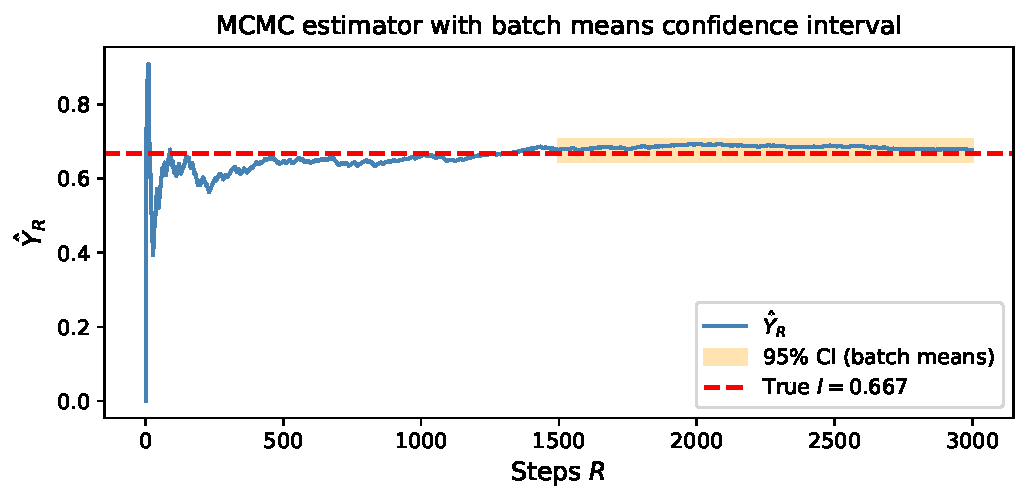
\includegraphics[width=0.7\linewidth]{fig_batch_means}
\end{frame}

\begin{frame}[fragile]{6.7 MCMC Estimation: Python Implementation}
\begin{lstlisting}[style=python]
import numpy as np
from scipy import stats

def mcmc_estimate_with_CI(chain_values, burn_in=500, n_batches=20):
    """
    Estimate I = E[f(X)] with 95% confidence interval via batch means.
    chain_values: array of f(X_j) values from MCMC chain
    """
    Y = chain_values[burn_in:]       # discard burn-in
    R = len(Y)
    I_hat = Y.mean()

    # Batch means
    batch_size = R // n_batches
    batches = [Y[k*batch_size:(k+1)*batch_size].mean() for k in range(n_batches)]
    batch_std = np.std(batches, ddof=1)

    # t-interval
    t_crit = stats.t.ppf(0.975, df=n_batches - 1)
    margin = t_crit * batch_std / np.sqrt(n_batches)

    # Asymptotic variance estimate via lag-k covariances
    N = 250   # truncation lag
    Y_c = Y - I_hat
    rho_hat = np.array([np.mean(Y_c[:R-k] * Y_c[k:]) for k in range(N+1)])
    zeta2_hat = rho_hat[0] + 2 * rho_hat[1:].sum()

    return {
        'estimate': I_hat,
        'CI_lower': I_hat - margin,
        'CI_upper': I_hat + margin,
        'zeta2_hat': zeta2_hat,
    }

# Hard-core model example: estimate mean particle count
np.random.seed(42)
n_grid = 8
# ... (run Gibbs sampler for hard-core model, collect f(xi) = sum(xi))
f_vals = np.random.normal(25, 3, 3000)  # placeholder for chain values
result = mcmc_estimate_with_CI(f_vals)
print(f"I_hat = {result['estimate']:.3f}")
print(f"95% CI = ({result['CI_lower']:.3f}, {result['CI_upper']:.3f})")
print(f"TAVC estimate zeta^2 = {result['zeta2_hat']:.4f}")
\end{lstlisting}
\end{frame}

% ============================================================
\section{6.8 Stable Simulation Scheme}
% ============================================================

\begin{frame}[allowframebreaks]{6.8 Stable Simulation Scheme (Siegmund Duality)}
  \textbf{Goal:} Estimate $\pi(A) = \sum_{s \in A}\pi_s$ for a \textbf{down-set} $A = \{s\}^\downarrow = \{s' \in \mathcal{S} : s' \preceq s\}$.

  \medskip
  \textbf{Setting:} $\mathcal{S} = \{s_1,\ldots,s_m\}$ partially ordered by $\preceq$; ergodic chain $(X_n)$ with stationary $\pi$.

  \begin{block}{Definition 6.8.1 (Siegmund Dual)}
    The Markov chain $(Z_n)$ with transition matrix $\mathbf{P}_Z$ is the \textbf{Siegmund dual} of $(X_n)$ if
    \[
      \forall\,(s_i, s_j) \in \mathcal{S},\; \forall n \ge 0: \quad
      \mathbf{P}_X^n(s_i, \{s_j\}^\downarrow) = \mathbf{P}_Z^n(s_j, \{s_i\}^\uparrow).
    \]
    Taking $n \to \infty$:
    \[
      \pi(\{s_j\}^\downarrow) = \PP(Z \text{ is absorbed in } s_m \mid Z_0 = s_j).
    \]
  \end{block}

  \framebreak

  \begin{block}{Key Formula (Eq.\ 6.8.2)}
    \[
      \pi(\{s_j\}^\downarrow) = \lim_{n\to\infty}\mathbf{P}_Z^n(s_j, \{s_i\}^\uparrow) = \PP(Z \text{ absorbed at } s_m \mid Z_0 = s_j).
    \]
    This relates the stationary distribution of $(X_n)$ to \textbf{absorption probabilities} of $(Z_n)$.
  \end{block}

  \begin{block}{Algorithm 59 (Stable Simulation Scheme)}
    \textbf{Require:} Möbius monotone chain $(X_n)$; set $\{s\}^\downarrow$; $R$ replications.
    \begin{enumerate}
      \item Compute Siegmund dual $Z$ of $X$ on $\mathcal{S}^* = \{s_0\} \cup \mathcal{S}$.
      \item For $j = 1,\ldots,R$: simulate $Z^{(j)}$ starting at $s$, until absorption.
      \item Estimate
            \[
              \hat{\pi}(\{s\}^\downarrow) = \frac{1}{R}\sum_{j=1}^R \mathbf{1}(Z^{(j)} \text{ absorbed at } s_m).
            \]
    \end{enumerate}
    Required replications: $R \approx b^{-2}$ where $b$ = desired half-width.
  \end{block}

  \framebreak

  \begin{block}{Definition 6.8.1 (Möbius Monotonicity)}
    Chain $(X_n)$ with t.m.\ $\mathbf{P}_X$ is \textbf{Möbius monotone} w.r.t.\ $\preceq$ if
    \[
      \mathbf{C}^{-1}\mathbf{P}_X\mathbf{C} \ge 0,
    \]
    where $\mathbf{C}(s_i, s_j) = \mathbf{1}(s_i \preceq s_j)$ is the \textbf{ordering matrix} and $\mathbf{C}^{-1}$ is the \textbf{Möbius function}.
  \end{block}

  \begin{block}{Lemma 6.8.2}
    There exists a Siegmund dual $Z$ of $X$ on $\mathcal{S}^* = \{s_0\} \cup \mathcal{S}$ if and only if $(X_n)$ is Möbius monotone w.r.t.\ $\preceq$.
  \end{block}

  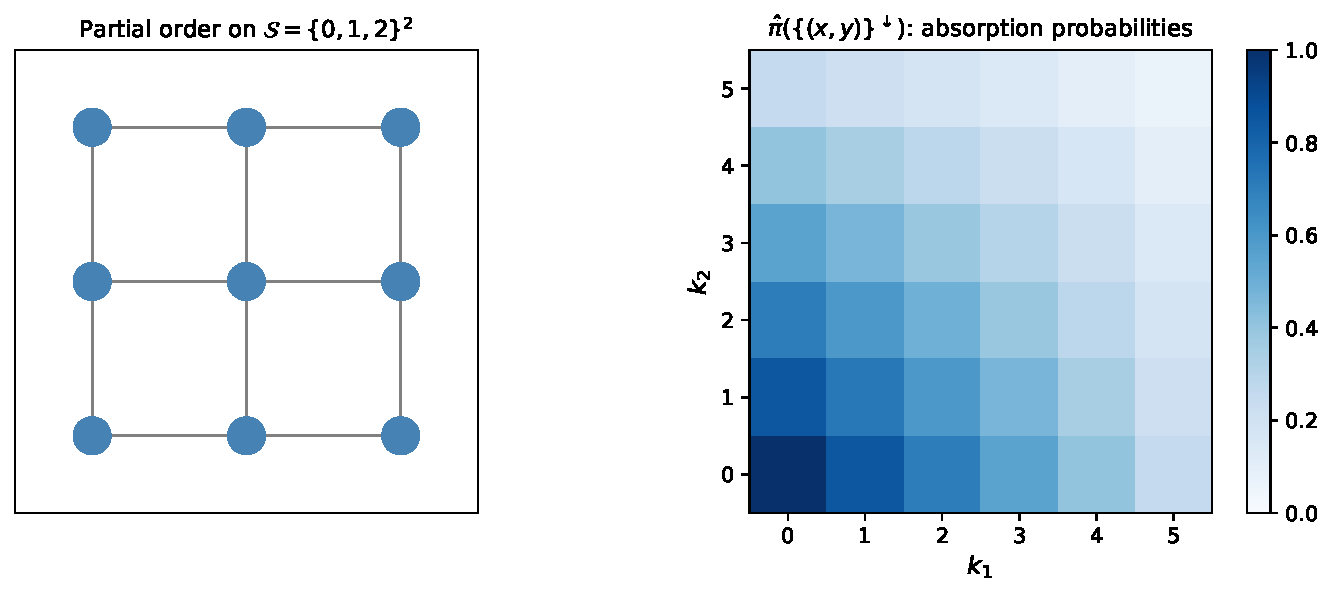
\includegraphics[width=0.7\linewidth]{fig_siegmund_duality}
\end{frame}

\begin{frame}{6.8 Tandem Queue Example (Example 6.8.4)}
  \textbf{Setup:} Two-node closed tandem queue, $\mathcal{S} = \{0,\ldots,N\}^2$, parameters $\lambda_1, \lambda_2, \mu_1, \mu_2$ with $\lambda_1 + \mu_1 + \lambda_2 + \mu_2 = 1$.

  \textbf{Goal:} Estimate $\pi(\{(x,y)\}^\downarrow) = \pi(\{(x',y') : x' \le x, y' \le y\})$ for all $(x,y) \in \mathcal{S}$.

  \begin{block}{Results ($N=5$, $\lambda_1=3/16$, $\lambda_2=1/16$, $\mu_1=\mu_2=6/16$, $R=4\cdot10^4$)}
    \begin{center}
    \footnotesize
    \begin{tabular}{c|cccccc}
      \toprule
      $y \backslash x$ & 0 & 1 & 2 & 3 & 4 & 5 \\
      \midrule
      0 & 0.030 & 0.081 & 0.145 & 0.236 & 0.351 & 0.502 \\
      1 & 0.058 & 0.139 & 0.249 & 0.381 & 0.550 & 0.763 \\
      2 & 0.079 & 0.181 & 0.310 & 0.468 & 0.652 & 0.884 \\
      3 & 0.094 & 0.207 & 0.353 & 0.511 & 0.710 & 0.946 \\
      4 & 0.102 & 0.224 & 0.372 & 0.540 & 0.743 & 0.981 \\
      5 & 0.111 & 0.235 & 0.383 & 0.558 & 0.762 & 1.000 \\
      \bottomrule
    \end{tabular}
    \end{center}
    Final 95\% CI for $\hat{Y}_R$ (starting from $k_0 = 500$, $N=250$): $(23.15, 25.59)$.
  \end{block}
\end{frame}

% ============================================================
\section{6.9 Bibliographical Notes}
% ============================================================

\begin{frame}{6.9 Bibliographical Notes (Summary)}
  \begin{itemize}
    \item \textbf{Markov chains:} Classical references include Norris [165], Meyn \& Tweedie [147].
    \item \textbf{Metropolis algorithm:} Metropolis \emph{et al.}\ [145] (1953); generalized by Hastings [78] (1970).
    \item \textbf{Gibbs sampler:} Introduced by Geman \& Geman [62] for image restoration; popularized in statistics by Gelfand \& Smith [61].
    \item \textbf{CFTP:} Propp \& Wilson [170] (1996); monotone CFTP by Huber [85].
    \item \textbf{Approximate counting / FPRAS:} Jerrum, Valiant \& Vazirani [100]; Dyer \emph{et al.}\ [43].
    \item \textbf{Motif finding:} Lawrence \emph{et al.}\ [119]; Gibbs approach by Liu \emph{et al.}\ [128].
    \item \textbf{Ergodic theorem / CLT for MC:} Meyn \& Tweedie [147]; Glynn \& Iglehart [64].
    \item \textbf{Batch means:} Damerdji [30]; Alexopoulos \& Seila [4].
    \item \textbf{Siegmund duality / stable simulation:} Siegmund [191]; Lorek \& Szekli [130].
  \end{itemize}
\end{frame}

% ============================================================
\section{6.10 Exercises (Selected)}
% ============================================================

\begin{frame}[allowframebreaks]{6.10 Selected Exercises}
  \begin{block}{Exercise 6.T.1 (Stationary distribution)}
    Find the stationary distribution of the Markov chain with transition matrix
    \[
      \mathbf{P} = \begin{pmatrix} r_0 & p_0 & 0 & \cdots & 0 & q_0 \\ q_1 & r_1 & p_1 & \cdots & 0 & 0 \\ \vdots & & \ddots & & & \vdots \\ p_N & \cdots & 0 & q_N & r_N \end{pmatrix}.
    \]
    \textit{Hint:} Use the detailed balance condition.
  \end{block}

  \begin{block}{Exercise 6.T.8 (Total variation distance)}
    Show that $\dTV(\bfmu, \bfv) = \max_{A \subseteq \mathcal{S}}|\mu(A) - \nu(A)|$.
  \end{block}

  \framebreak

  \begin{block}{Exercise 6.T.12 (Two-state weather chain)}
    Chain on $\mathcal{S} = \{\text{rainy}, \text{sunny}\}$ with $\mathbf{P} = \begin{pmatrix}1/2 & 1/2 \\ 1/10 & 9/10\end{pmatrix}$.
    \begin{enumerate}[(a)]
      \item Find the stationary distribution.
      \item Starting from ``rainy'', compute $\dTV(\bfmu\mathbf{P}^n, \pi)$ for $n = 1, 2, 3$.
    \end{enumerate}
  \end{block}

  \begin{block}{Exercise 6.T.35 (Median trick for boosting)}
    Show that if $p > 1/2$ and $S_R = \sum_{i=1}^R Y_i$ where $Y_i \sim \text{Bernoulli}(p)$, then
    \[
      \PP(S_R > R/2) \ge 1 - \delta \quad \text{for } R = \frac{\log(1/\delta) \cdot 2p}{(p-1/2)^2}.
    \]
    (This is used in the FPRAS boosting lemma.)
  \end{block}
\end{frame}

% ============================================================
% Summary
% ============================================================

\begin{frame}{Chapter 6 Summary}
  \begin{columns}[T]
    \begin{column}{0.5\textwidth}
      \textbf{Key Algorithms:}
      \begin{itemize}
        \item \textbf{Metropolis-Hastings} (Alg.\ 42--43): accept/reject with ratio $\pi_{s'}/\pi_s$.
        \item \textbf{Gibbs sampler} (Alg.\ 44--48): sample one coordinate from full conditional.
        \item \textbf{CFTP} (Alg.\ 50--53): perfect simulation via monotone coupling.
        \item \textbf{FPRAS} (Alg.\ 54--55): approximate counting via telescoping ratios.
        \item \textbf{Stable simulation} (Alg.\ 59): Siegmund duality for $\pi(A)$.
      \end{itemize}
    \end{column}
    \begin{column}{0.47\textwidth}
      \textbf{Key Theory:}
      \begin{itemize}
        \item Detailed balance $\Rightarrow$ stationary $\pi$.
        \item Ergodic theorem: $\hat{Y}_R \to I$ a.s.
        \item CLT: $\sqrt{R}(\hat{Y}_R - I) \to \mathcal{N}(0, \varsigma^2)$.
        \item TAVC $\varsigma^2$: estimate via covariances or batch means.
        \item FPRAS requires $\varrho_i \ge 1/2$ and rapid mixing.
        \item CFTP: monotone $\Rightarrow$ coalescence $\Rightarrow$ exact sample from $\pi$.
      \end{itemize}
    \end{column}
  \end{columns}

  \bigskip
  \begin{center}
    \textbf{The MCMC paradigm}: Build a chain with stationary $\pi$ $\to$ run it $\to$ average.
  \end{center}
\end{frame}

\end{document}
